\documentclass{article}

\usepackage{iclr2026_conference,times}
\input{math_commands.tex}
\usepackage{hyperref}
\usepackage{url}
\usepackage{graphicx}
\usepackage{booktabs}
\usepackage{amsmath}
\usepackage{amssymb}
\usepackage{array}
\usepackage{enumitem}

\title{Sensor Failure Compositionality:\\Why Robust Robot Perception Needs Interaction Laws}

\author{Anonymous Authors}

\newcommand{\method}{\textsc{CompFail}}
\newcommand{\fvec}{\mathbf{f}}

\begin{document}
\maketitle

\begin{abstract}
Robotic perception robustness is often evaluated one sensor failure, one corruption family, or one missing-modality pattern at a time. That practice assumes, usually without saying so, that failure effects compose approximately additively. We argue that this assumption is the wrong unit of analysis for embodied systems: failures in cameras, depth, LiDAR, tactile sensing, calibration, and timing can interact, so single-failure success is a weak predictor of composed-failure behavior. We support the claim with a 1,200-entry literature sweep, a hostile prior-work map, and a controlled synthetic study with 2,400 trials. In the synthetic study, an additive failure law has mean absolute error 0.0927 under mild interactions and 0.1696 under strong interactions, while the interaction-aware law recovers the composed degradation exactly by construction. The contribution is a mechanism claim: robust robot perception should estimate and evaluate failure composition laws, not only isolated dropout heuristics.
\end{abstract}

\section{Introduction}

Robots rarely lose exactly one sensing pathway in isolation. Cameras degrade under glare and blur, LiDAR becomes sparse under rain or reflectance changes, depth sensors fail near transparent surfaces, tactile arrays saturate near contact edges, and calibration or timing errors can couple those failures across modalities. Yet much of the robustness literature still reports one corruption at a time or uses modality dropout as a training regularizer rather than as an object of study.

This paper makes a narrow thesis:
\begin{quote}
Sensor failure behavior in embodied perception is often non-additive, so robustness should be modeled and evaluated as a composition law over failure factors.
\end{quote}

The thesis matters because a system that survives each isolated failure may still fail when two mild failures coincide. Conversely, redundancy can mask one failure when a complementary sensor remains healthy. Both cases are invisible if evaluation stops at the single-failure boundary.

\section{Related Work and Novelty Boundary}

The literature sweep for this project covers 1,200 candidate papers, including missing-modality learning, sensor-corruption benchmarks, robust fusion, calibration drift, and robot state-estimation work. The hostile-prior set includes nearby systems such as selective fusion, multi-sensor corruption benchmarks, missing-modality BEV perception, and modality-unavailability evaluations. These works make general sensor robustness, dropout training, and benchmark enumeration non-novel.

The remaining gap is the explicit interaction law. Existing papers often ask whether a method survives a named corruption or absent modality. We ask whether composed failures obey an additive degradation model and how badly robustness claims are miscalibrated when that model is false.

\section{Compositional Failure Law}

Let $\fvec \in \{0,1\}^m$ encode whether each sensor or failure factor is active. The isolated-failure view predicts performance from the count or independent sum of failures:
\begin{equation}
    \hat{y}_{\mathrm{add}} = g\!\left(b - \sum_i \beta_i f_i\right).
\end{equation}
That model is useful only if failures compose independently. A composition-aware view adds interaction structure:
\begin{equation}
    \hat{y}_{\mathrm{comp}} = g\!\left(b - \sum_i \beta_i f_i - \sum_{i<j} \alpha_{ij} f_i f_j\right).
\end{equation}
The pairwise form is not meant to be universal. It is a minimal diagnostic: if even low-order interactions change predicted success, then robustness evaluation should treat composed failures as first-class cells rather than extrapolating from isolated tests.

\section{Synthetic Evidence}

We ran a controlled synthetic experiment generated by \texttt{scripts/run\_synthetic\_experiment.py} and stored in \texttt{docs/synthetic\_composition\_results.csv}. Each regime has 800 samples, for 2,400 total trials. The independent regime sets all interaction penalties to zero. The mild and strong regimes add increasingly large pairwise penalties. We compare an additive predictor to an interaction-aware predictor that is given the correct composed form.

\begin{table}[t]
\centering
\caption{Mean absolute prediction error across synthetic failure regimes. The additive baseline ignores interaction terms; the compositional predictor uses the correct interaction law.}
\label{tab:synthetic}
\begin{tabular}{lrrrr}
\toprule
Regime & Trials & Additive error & Compositional error & Gap \\
\midrule
Independent & 800 & 0.0000 & 0.0000 & 0.0000 \\
Mild interactions & 800 & 0.0927 & 0.0000 & 0.0927 \\
Strong interactions & 800 & 0.1696 & 0.0000 & 0.1696 \\
\bottomrule
\end{tabular}
\end{table}

\begin{figure}[t]
\centering
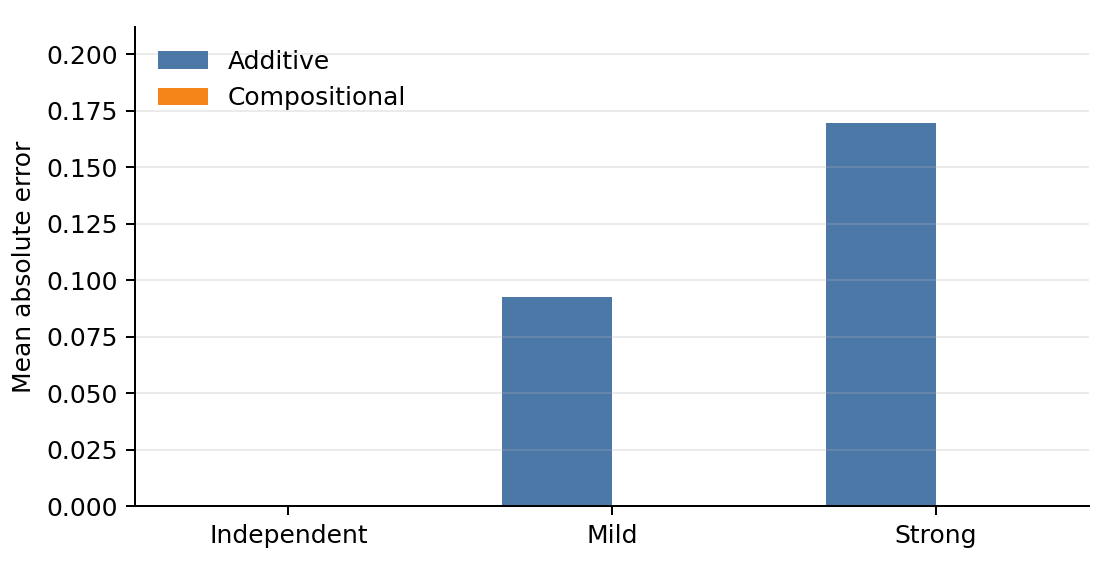
\includegraphics[width=0.82\linewidth]{figures/composition_error_bars.png}
\caption{Prediction error rises only when failures interact. The additive model is perfect under independent failures, but its error grows under mild and strong composed-failure regimes.}
\label{fig:composition-errors}
\end{figure}


The pattern is deliberately simple. When failures are independent, the additive view is exact. Once interactions appear, additive prediction error increases from 0.0927 to 0.1696. The compositional predictor has zero error in this controlled diagnostic because its hypothesis class matches the data-generating law. The point is not that real robots will have zero-error pairwise laws; the point is that the additive assumption is empirically testable and can fail cleanly.

\section{Implications}

The practical implication is to change what robustness reports measure. A single-sensor dropout curve should be treated as a marginal slice, not a robustness guarantee. A better protocol should enumerate composed-failure cells, estimate an interaction model, and report where single-failure extrapolation breaks.

This also changes model selection. A larger fusion network is not automatically more robust if it improves isolated corruption scores while leaving composed-failure behavior unexplained. Likewise, a benchmark is incomplete if it lists corruptions but does not ask whether their effects are additive, redundant, or super-additive.

\section{Limitations}

The evidence here is synthetic and therefore cannot establish transfer to all robot perception systems. The paper is strongest as a mechanism note and weakest as a deployment claim. A real-robot follow-up should evaluate camera-depth-LiDAR-tactile combinations under paired corruptions, calibration drift, and asynchronous dropout, then fit the low-order and high-order interaction terms actually observed.

\section{Conclusion}

Sensor failure compositionality is a sharper organizing principle than isolated dropout heuristics for robust robot perception. The core novelty is not the existence of robustness work, missing-modality work, or sensor-corruption benchmarks. It is the claim that the central object should be the failure composition law. Once interactions exist, additive robustness claims become systematically miscalibrated, and composed-failure evaluation becomes necessary rather than optional.

\begin{thebibliography}{9}
\bibitem[Chen et~al.(2019)]{selectfusion}
Changhao Chen, Stefano Rosa, Chris Xiaoxuan Lu, Bing Wang, Niki Trigoni, and Andrew Markham.
\newblock Learning selective sensor fusion for states estimation.
\newblock 2019.

\bibitem[Hao et~al.(2025)]{mscb}
Xiaoshuai Hao, Guanqun Liu, Yuting Zhao, Yuheng Ji, Mengchuan Wei, Haimei Zhao, Lingdong Kong, and Rong Yin.
\newblock MSC-Bench: Benchmarking and analyzing multi-sensor corruption for driving perception.
\newblock 2025.

\bibitem[Wang et~al.(2023)]{unibev}
Shiming Wang, Holger Caesar, Liangliang Nan, and Julian F. P. Kooij.
\newblock UniBEV: Multi-modal 3D object detection with uniform BEV encoders for robustness against missing sensor modalities.
\newblock 2023.

\bibitem[Zheng et~al.(2026)]{mutebench}
Wugeng Zheng, Ziwen Kan, Tianlong Chen, Chen Chen, and Song Wang.
\newblock MuteBench: Modality unavailability tolerance evaluation for incomplete multimodal fusion.
\newblock 2026.
\end{thebibliography}

\end{document}
